% SIAM Article Template
\documentclass[review]{siamonline1116}

% Information that is shared between the article and the supplement
% (title and author information, macros, packages, etc.) goes into
% ex_shared.tex. If there is no supplement, this file can be included
% directly.

% SIAM Shared Information Template
% This is information that is shared between the main document and any
% supplement. If no supplement is required, then this information can
% be included directly in the main document.


% Packages and macros go here
\usepackage{lipsum}
\usepackage{amsfonts}
\usepackage{graphicx}
\usepackage{epstopdf}
\usepackage{algorithmic}
\ifpdf
  \DeclareGraphicsExtensions{.eps,.pdf,.png,.jpg}
\else
  \DeclareGraphicsExtensions{.eps}
\fi

%strongly recommended
\numberwithin{theorem}{section}

% Declare title and authors, without \thanks
\newcommand{\TheTitle}{An Example Article} 
\newcommand{\TheAuthors}{D. Doe, P. T. Frank, and J. E. Smith}

% Sets running headers as well as PDF title and authors
\headers{\TheTitle}{\TheAuthors}

% Title. If the supplement option is on, then "Supplementary Material"
% is automatically inserted before the title.
\title{{\TheTitle}\thanks{Submitted to the editors DATE.
\funding{This work was funded by the Fog Research Institute under contract no.~FRI-454.}}}

% Authors: full names plus addresses.
\author{
  Dianne Doe\thanks{Imagination Corp., Chicago, IL
    (\email{ddoe@imag.com}, \url{http://www.imag.com/\string~ddoe/}).}
  \and
  Paul T. Frank\thanks{Department of Applied Mathematics, Fictional
    University, Boise, ID (\email{ptfrank@fictional.edu},
    \email{jesmith@fictional.edu}).}
  \and
  Jane E. Smith\footnotemark[3]
}

\usepackage{amsopn}
\DeclareMathOperator{\diag}{diag}


%%% Local Variables: 
%%% mode:latex
%%% TeX-master: "ex_article"
%%% End: 


% Optional PDF information
\ifpdf
\hypersetup{
  pdftitle={\TheTitle},
  pdfauthor={\TheAuthors}
}
\fi

% The next statement enables references to information in the
% supplement. See the xr-hyperref package for details.

\externaldocument{ex_supplement}

% FundRef data to be entered by SIAM
%<funding-group>
%<award-group>
%<funding-source>
%<named-content content-type="funder-name"> 
%</named-content> 
%<named-content content-type="funder-identifier"> 
%</named-content>
%</funding-source>
%<award-id> </award-id>
%</award-group>
%</funding-group>


\title{Parameter Estimation for JSPAM Galaxtic Merger Simulations}
\author{John Wallin, Graham West}


\begin{document}

\maketitle

% REQUIRED
\begin{abstract}
In this paper, we present the implementation and results of an MCMC-type optimization method to solve the problem of estimating dynamical parameters of galaxy mergers. Using a Metropolis-Hastings algorithm with adaptive step-sizes along with the appropriate fitness function, we are able to find a merger simulation of minimum error with respect to a given merger target.
\end{abstract}

% REQUIRED
\begin{keywords}
galaxy mergers, MCMC, optimization, simulation, n-body
\end{keywords}

% REQUIRED
\begin{AMS}
  68Q25, 68R10, 68U05
\end{AMS}

\section{Introduction}
Understanding the morphology and evolution of galactic mergers is a central issue facing modern astrophysicists--in particular, the inverse problem of tracing a merger back in time. Since this problem cannot be solved by simply reversing time in an n-body simulation, one must use optimization algorithms which necessitate the simulation of a great number of mergers to fully explore the parameter space.

In order for this to be done efficiently we need three things: 1) a fast simulation code, 2) a fitness function which accurately measures the error between two mergers, and 3) an optimization algorithm which can minimize???? the fitness function. Step 1 was completed by Wallin et al. \cite{jspam} with the development of the Fortran simulation code entitled JSPAM (\_\_\_\_). We have been developing steps 2 and 3 simultaneously due to the fact that different fitness functions yield different behaviours in the parameter search process.

In what follows, we will discuss the tools and data we had at our disposal, including JSPAM, \textit{Merger Wars} and \textit{Galaxy Zoo: Mergers}, and the SDSS and MaNGA surveys. Then--in the majority of the paper--we will examime our method of calculating the fitness function and the MCMC algorithm which optimizes it. Lastly, we will explore several key next steps which we will take to integrate the MaNGA data into our process so that we can begin fitting real mergers.

% These aren't necessarily steps, so that might not be the right word

\subsection{JSPAM}

Due to the nature of gravitation being a pair-wise interaction and the structure of galaxies being essentially a cloud of massive particles--which is true as far as many computer models are concerned--the most direct way to simulate a merger would be to set up a full $O(n^2)$ n-body code. Approximations can be made which reduce the complexity to $O(n\hspace{1pt}$log$(n))$--hierarchical tree codes, for example--but, even this is too slow for our purposes. Due to the great quantity of simulations needed to be performed, we required a code which was $O(n)$. Thus, we used the restricted three-body JSPAM Fortran code developed by Wallin et al. \cite{jspam}.

This code makes several significant simplifications for the sake of runtime, but since the mergers are not simulated over a long time interval, accuracy is retained. Within the code, galaxies themselves are comprised of two parts: a center of mass and a swarm of massless particles. The massless particles only interact with the centers of mass of the two galaxies while the centers of mass only interact with each other. The reference frame of the simulation is setup so that one galaxy (called the primary) is initially at the origin with zero velocity and the other galaxy (called the secondary) is given a relative position and velocity. The list of dynamical parameters which describe the merger include these relative positions and velocities, the masses of the galaxies, their radii, and their orientations in terms of altitude and azimuth w.r.t. the $z$-axis.

\begin{figure}[!h]
	\centering
	\begin{align*}
		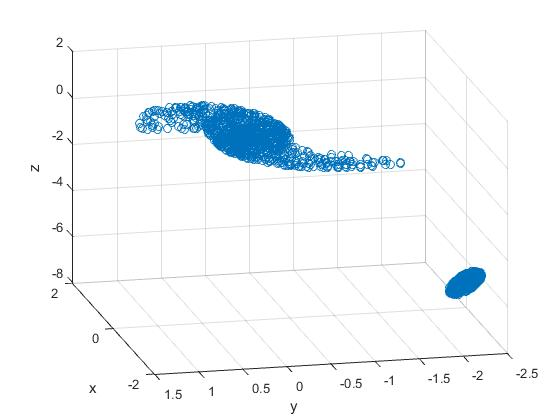
\includegraphics[scale = 0.35]{JSPAMTestPlot_xyz} & 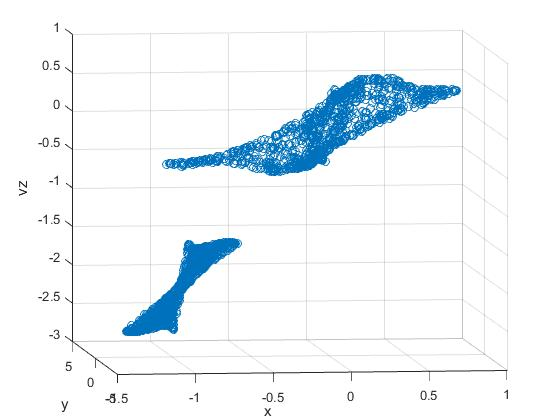
\includegraphics[scale = 0.35]{JSPAMTestPlot_xyvz}
	\end{align*}
	\caption{Final time-step of a JSPAM merger simulation (1000 particles per galaxy). Left: X-Y-Z plot. Right X-Y-Vz plot. NOTE: the graphs are viewed at two different orientations.}
\end{figure}

Given a list of \emph{final} parameters post-merger, the code integrates backward in time, past the point of closest approach to a fixed starting time. After this point, there are several initialization steps, including particle positions/velocities and the galactic potential. Since the galactic potential is a fairly complicated function which must be called many times throughout a simulation, it is assumed to be spherically symmetric, pre-calculated at a set of fixed radial distances, and stored. During simulations, the value of the potential in between these radii is calculated via linear interpolation.

Since the potentials are stored, they do not change over time; however, since they originate from the centers of mass, they do translate through space. In addition to the potential, particles also experience a force due to dynamical friction. This phenomenon slows objects traveling through a medium of gravitating particles by causing an increase in particle density behind the object, thus increasing the gravitational force in the retrograde direction.

\subsection{Merger Wars and Galaxy Zoo: Mergers}

From a computational perspective, the problem of finding an appropriate fitness function for comparing morphologies is a real challenge. It is difficult to find a method that is robust enough to perform on a level equivalent to that of a human. By nature, humans are excellent at pattern recognition; and where it can be difficult to ``train'' an algorithm to spot similarities between objects, humans can do it almost instinctively. For this reason, Holincheck et al. \cite{citizen} employed the help of thousands of Citizen Scientists to assist the \emph{Galaxy Zoo: Mergers} project in which they volunteered their pattern recognition abilities to determine best-fit models for 62 actual mergers.

The volunteers analyzed the morphologies of many thousands of simulations via a vote-based tournament scheme called the \emph{Merger Wars} algorithm. In a typical session, a volunteer is shown an image of the target (the actual merger) along with two simulations which model the target. The volunteer then chooses which simulation is most similar to the target, which counts as a ``win'' for one and a ``loss'' for the other. (They can also select neither image, thereby affording both images a loss.) Since it is entirely possible for images to be judged poorly, every simulation participates in multiple rounds of the tournament so that a bad round does not have a large impact on the results of the competition. The fitness of a particular simulation is then calculated as the percentage of ``wins'' it achieved, with the maximum being 1. Since an integral part of our research involved find an explicit mathematical fitness function for the merger morphologies, it was very useful to have the \emph{Merger Wars} data with which we could assess the validity of our own data.

\subsection{SDSS and MaNGA}
The end goal of our research is to construct an automated pipeline which can compare the morphologies of simulated mergers with images of actual mergers. Once we reach this stage, we will use the Sloan Digital Sky Survey's (SDSS) extensive catalog of observational data. Over the years, SDSS has provided many large, detailed data releases on collections of galactic mergers, the latest of which includes data from the Mapping Nearby Galaxies at APO (MaNGA) project. Thanks to the use of new observational tools, MaNGA has been able to capture spectra over the surface of nearly 2,000 galaxies, including many mergers. With this information, it is possible to derive the velocity fields and dispersions of the galaxies and using these velocity fields, we will be able to apply our morphological fitness functions.





\section{Objective Function}
\label{sec:alg}

Stuff

\subsection{Binning}



\subsection{Calculating Error}





\section{Conclusions}
\label{sec:conclusions}

Some conclusions here.


\appendix
\section{An example appendix} 
\lipsum[71]

\section*{Acknowledgments}
We would like to acknowledge the assistance of volunteers in putting
together this example manuscript and supplement.

\bibliographystyle{siamplain}
\bibliography{references}



\begin{thebibliography}{10}

\bibitem{citizen} A. Holincheck, J. Wallin, K. Borne, L. Fortson, C. Lintott, A M. Smith, S. Bamford, W. Keel, and M. Parrish, ``Galaxy Zoo: Mergers - Dynamical Models of Interacting Galaxies.'' \textit{MNRAS}, (2016). Vol. 459, Is. 1, 720-745.

\bibitem{galaxyFE} H. Mo, F. Bosch, and S. White, \textit{Galaxy Formation and Evolution}, 2010, Cambridge University Press.

\bibitem{jspam} J. Wallin, A. Holincheck, and A. Harvey, ``JSPAM: A restricted three-body code for simulating interacting galaxies.'' \textit{Astronomy and Computing} 16, (2016). 26-33.


\end{thebibliography}


\end{document}




